\subsection{C7 -- Brownian bacteria ominion window}\label{suppc:c7-brownian-bacteria}
\paragraph{Question.} Does a cited bacteria ominion window show the predicted mass-scaled loss/tension burden, dominant residual-duration support, cadence-noise band, and recurrent drift profile when compared against familiar Brownian/motility observations?

\paragraph{Cited input block.} Familiar observational context is anchored to bacterial Brownian/motility studies near surfaces and in suspension.\footnote{G. Li and J. X. Tang, \href{https://pmc.ncbi.nlm.nih.gov/articles/PMC2587629/}{Amplified effect of Brownian motion in bacterial near-surface swimming}, \emph{PNAS} \textbf{106} (2009); M. D. Manson, \href{https://pmc.ncbi.nlm.nih.gov/articles/PMC7648147/}{Howard Berg's Random Walk through Biology}, \emph{PNAS} \textbf{117} (2020).} For the rendered mass anchor, single-cell bacterial dry-mass measurements and the corresponding dry-mass/volume allometry are taken from Loferer-Kroessbacher, Klima, and Psenner and the BioNumbers digest of that work.\footnote{M. Loferer-Kroessbacher, J. Klima, and R. Psenner, \href{https://pmc.ncbi.nlm.nih.gov/articles/PMC106103/}{Determination of bacterial cell dry mass by transmission electron microscopy and densitometric image analysis}, \emph{Appl. Environ. Microbiol.} \textbf{64} (1998); BioNumbers, \href{https://bionumbers.hms.harvard.edu/bionumber.aspx?id=106616&s=n&v=0}{Correlation between dry weight and bacterial cell volume}.}

\paragraph{Declared reduction.} The bacterium is reduced to the cited ominion
\[
O_{\mathrm{bacteria}}(\omega),
\]
carrying effective mass/rate, phase state, and loss/tension witnesses on the cited jitter window. The row is keyed as
\[
\texttt{tetron:*:[bacteria]:6},
\]
so the clustered body is retained explicitly and the shell/chirality support is not flattened into a 2D jitter placeholder.

\paragraph{Readout.}
\begin{itemize}
\item cited object $O_{\mathrm{bacteria}}$
\item cited window $\omega_{\mathrm{jit,bac}}$
\item structural key \texttt{tetron:*:[bacteria]:6}
\item frame count / $T_{\mathrm{eval}}=1024$ bip
\item weighting policy $w(\kappa)\equiv 1$
\item jitter/dwell samples on the same cited window
\end{itemize}

\paragraph{Operator chain.}
\[
m_{\mathrm{eff}}
\to
m_z
\to
R_{\mathrm{loss}}
\to
b(\kappa)
\to
H_B
\to
B^*
\to
\Lambda_b
\to
\text{cadence-noise witness},\ \text{drift witness}.
\]

\paragraph{Output row.}
\begin{center}
\begin{tabularx}{\linewidth}{@{}lXcccll@{}}
\toprule
Row & Structural key & $B^*$ & $\Lambda_b$ & $R_{\mathrm{loss}}$ [trit/bip] & Cadence-noise & Drift \\
\midrule
C7.A & \shortstack[l]{\texttt{tetron:*:}\\\texttt{[bacteria]:6}} & \textbf{2} & \textbf{11} & mass-scaled service burden & jitter band & recurrent \\
\bottomrule
\end{tabularx}
\end{center}

\paragraph{Rendering block.} This test is retained in default-form units. The cited bacterial-motion and bacterial dry-mass sources provide observational and SI anchors only; the row itself is carried on the ominion loss/tension ledger.

\paragraph{Figure witness.}
\begin{figure}[H]
\centering
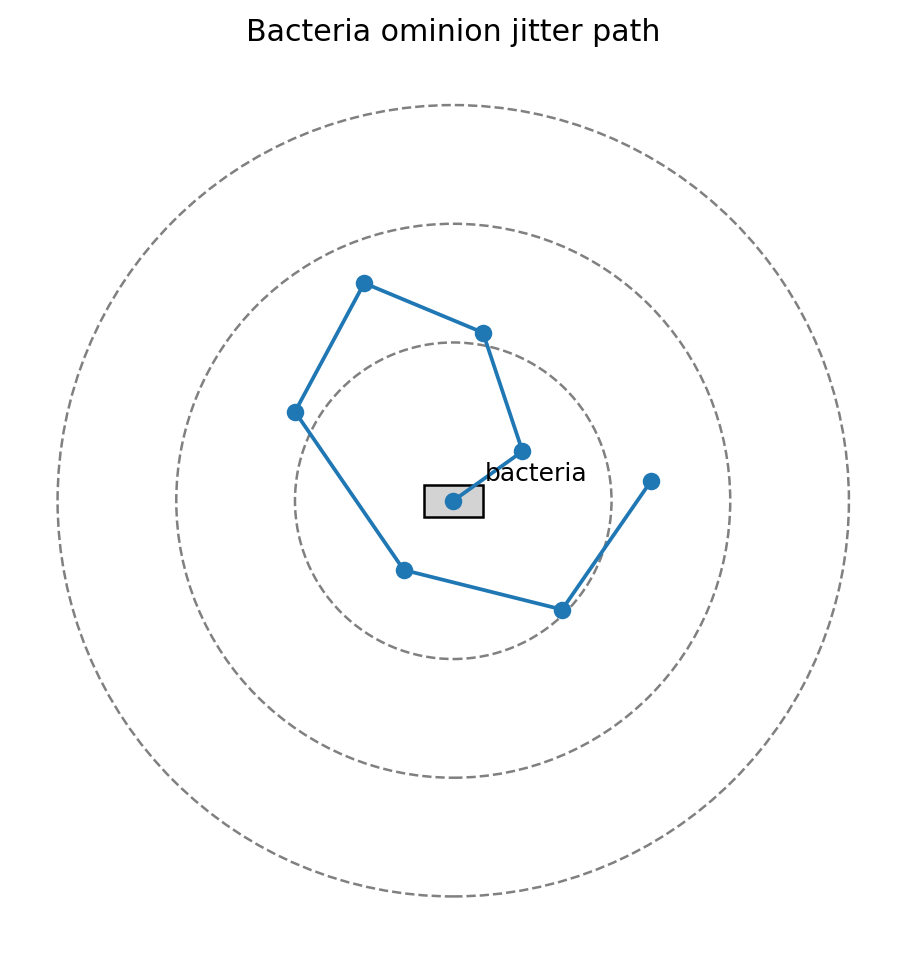
\includegraphics[width=0.66\linewidth]{figures/bacteria/bacteria_ominion_jitter.png}
\caption{Bacteria ominion jitter path with shell-like dwell bands. The notebook reproduces the same schematic and writes the canonical artifact into the supplement-wide figures directory.}
\end{figure}

\FloatBarrier

\paragraph{Hook / Evidence.} Use the cited recurrent-jitter and dwell-distribution hooks, now read on the bacteria ominion ledger.

\paragraph{Companion notebook and manifest.} See Section~\ref{app:suppc-notebooks} for the executed calculation manifest and generated figure provenance for this section.

\begin{quote}\small\path{notebooks/bacteria/c7_bacteria_ominion_worked.ipynb}\end{quote}
